\documentclass[answers]{exam}

\usepackage{amsmath}
\usepackage{amssymb}
\usepackage{geometry}
\usepackage{venndiagram}
\usepackage{graphics}
\usepackage{graphicx}
\usepackage{tikz}
\usetikzlibrary{shapes.geometric}

% Header and footer.
\pagestyle{headandfoot}
\runningheadrule
\runningfootrule
\runningheader{Applied Stochastic Processes}{Assignment 3}{Fall 2023 }
\runningfooter{}{Page \thepage\ of \numpages}{}
\firstpageheader{}{}{}

\boxedpoints
\printanswers

\newcommand{\uvec}[1]{\boldsymbol{\hat{\textbf{#1}}}}
\newcommand\union\cup
\newcommand\inter\cap
\newcommand\ul\underline
\newcommand\ol\overline

\title{Assignment 3\\ Applied Stochastic Processes\\ Habib University -- Fall 2023}
\author{Ali Asghar Yousuf - ay06993 \\ Muhammad Murtaza - mm06369 }  % replace with your ID, e.g. oy02945
\date{\today}

\begin{document}
\maketitle
\section{Bertsekas and Tsitsiklis, Section 7.1}
\begin{questions}
    \question \textbf{Problem 2}

    Dave fails quizzes with probability $\dfrac{1}{4}$, independent of other
    quizzes.
    \begin{parts}
        \part What is the probability that Dave fails exactly two of the next six quizzes?
        \begin{solution}
            \begin{align*}
                P(\text{Dave fails exactly two of the next six quizzes}) & = \binom{6}{2} \left(\frac{1}{4}\right)^2 \left(\frac{3}{4}\right)^4 \\
                                                                         & = 15 \times \frac{1}{16} \times \frac{81}{256}                       \\
                                                                         & = \frac{1215}{4096}                                                  \\
                                                                         & = 0.296875
            \end{align*}
        \end{solution}
        \part What is the expected number of quizzes that Dave will pass before he has failed
        three times?
        \begin{solution}

            No. of times he failed $= 3$ \\ Total no. of quizzes taken to fail 3 times $=
                n$ \\
            \begin{align*}
                n * \frac{1}{4} = 3 \\
                n = 12
            \end{align*}
            Dave takes 12 quizzes to fail 3 times. Therefore, he passes 9 quizzes. \\
        \end{solution}
        \part What is the probability that the second and third time Dave fails a quiz will
        occur when he takes his eighth and ninth quizzes, respectively?
        \begin{solution}

            1st Fail $\rightarrow 1 - 7$ quizzes \\
            2nd Fail $\rightarrow 8$th quiz \\
            3rd Fail $\rightarrow 9$th quiz \\

            \begin{align*}
                P(X) & =P(\text{1 fail in 7 tests}) \cdot P(\text{2nd fail in 8th test}) \cdot P(\text{3rd fail in 9th test}) \\
                     & =\binom{7}{1}\left(\frac{1}{4}\right)^1 \left(\frac{3}{4}\right)^6 \cdot \frac{1}{4} \cdot \frac{1}{4} \\
                     & =\frac{7 \cdot 3^6}{4^9} = \frac{5103}{262144}                                                         \\
                     & =0.0194568634
            \end{align*}
        \end{solution}
        \part What is the probability that Dave fails two quizzes in a row before he passes two
        quizzes in a row?
        \begin{solution}

            $F =$ Fail, $P =$ Pass \\
            \begin{align*}
                P(X) & = P(\text{Dave fails two quizzes in a row before he passes two quizzes in a row})                                                                                 \\
                     & = P(FF \cup PFF \cup FPFF \cup PFPFF \cup FPFPFF \cup \dots)                                                                                                      \\
                     & = \dfrac{[P(F)]^2}{1 - P(F) \cdot P(P)} + \dfrac{P(P) \cdot [P(F)]^2}{1 - P(F) \cdot P(P)}                                                                        \\
                     & = \dfrac{\left(\frac{1}{4}\right)^2}{1 - \frac{1}{4} \cdot \frac{3}{4}} + \dfrac{\frac{3}{4} \cdot \left(\frac{1}{4}\right)^2}{1 - \frac{1}{4} \cdot \frac{3}{4}} \\
                     & = \dfrac{7}{52}
            \end{align*}

        \end{solution}
    \end{parts}

    \question \textbf{Problem 3}

    A computer system carries out tasks submitted by two users. Time is divided
    into slots. A slot can be idle, with probability $P_I = \frac{1}{6}$, and busy
    with probability $P_B = \frac{5}{6}$. During a busy slot, there is probability
    $P_{1 | B} = \frac{2}{5}$ (respectively, $P_{2 | B} = \frac{3}{5}$) that a task
    from user 1 (respectively, 2) is executed. We assume that events related to
    different slots are independent. \\ $T_1 = $ Task from user 1.

    \begin{parts}
        \part Find the probability that a task from user 1 is executed for the first time during
        the 4th slot.
        \begin{solution}
            If a task from user 1 is executed for the first time during the 4th slot, then the task from user 1 is not executed in the first 3 slots
            (they are busy and not accepting from user 1) and is executed in the 4th slot (4th slot maybe idle and execute or busy and execute). \\
            \begin{align*}
                 & P(T_1 \text{ is executed for the first time during the 4th slot})                                                                                  \\
                 & = P(T_1 \text{ is not executed in the first 3 slots}) \cdot P(T_1 \text{ is executed in the 4th slot})                                             \\
                 & = \left(\frac{5}{6} \times \frac{3}{5}\right)^3 \cdot \left[\left(\frac{1}{6} \times 1\right) + \left(\frac{5}{6} \times \frac{2}{5}\right)\right] \\
                 & = \left(\frac{1}{2}\right)^3 \cdot \left[\frac{1}{6} + \frac{1}{3}\right]                                                                          \\
                 & = \frac{1}{8} \cdot \frac{1}{2}                                                                                                                    \\
                 & = \frac{1}{16}                                                                                                                                     \\
            \end{align*}
        \end{solution}

        \part Given that exactly 5 out of the first 10 slots were idle, find the probability that
        the 6th idle slot is slot 12.
        \begin{solution}
            Since exactly 5 out of the first 10 slots were idle, therefore, the 11th slot is busy. \\
            And since the slots are independent, \\
            \begin{align*}
                 & P(\text{6th idle slot is slot 12})                              \\
                 & = P(\text{11th slot is busy}) \cdot P(\text{12th slot is idle}) \\
                 & = \frac{5}{6} \times \frac{1}{6}                                \\
                 & = \frac{5}{36}                                                  \\
                 & = 0.138889
            \end{align*}
        \end{solution}

        \part Find the expected number of slots up to and including the 5th task from user 1.
        \begin{solution}
            Probability of a task from user 1.
            \begin{align*}
                P(T_1) & = P_I \cdot P_{1|I} + P_B \cdot P_{1|B}               \\
                       & = \frac{1}{6} \cdot 1 + \frac{5}{6} \cdot \frac{2}{5} \\
                       & = \frac{1}{6} + \frac{1}{3}                           \\
                       & = \frac{1}{2}
            \end{align*}
            Probability of 5th task from user 1 (first 4 slots are busy and not accepting from user 1).
            \begin{align*}
                P(\text{5th task from user 1}) & = \left(\frac{1}{2}\right)^5 \\
                                               & = \frac{1}{32}
            \end{align*}
            Expected number of slots up to and including the 5th task from user 1 is the reciprocal of the probability of 5th task from user 1 $= 32$
        \end{solution}
        \part Find the expected number of busy slots up to and including the 5th task from
        user 1.
        \begin{solution}
            In busy slots, there is probability $P_{1 | B} = \frac{2}{5}$ that a task from user 1 is executed. \\
            Probability of 5th task from user 1 $ = \left(\frac{5}{6}\right)^5 \cdot \frac{2}{5} = 0.16075$ \\
            Expected number of busy slots up to and including the 5th task from user 1 is the reciprocal of the probability of 5th task from user 1 $= \frac{1}{0.16075} = 6.219$
        \end{solution}

        \part Find the PMF, mean, and variance of the number of tasks from user 2 until the
        time of the 5th task from user 1.
        \begin{solution}
            \begin{align*}
                \binom{k+r-1}{k} p^{k} (1-p)^{r}                                                              \\
                p               & = \left( \frac{1}{6} + \frac{5}{6} \times \frac{3}{5} \right) = \frac{2}{3} \\
                \binom{k+r-1}{k} \left(\frac{2}{3}\right)^{k} \left(\frac{1}{3}\right)^{r}                    \\
                \text{Mean}     & = \frac{pr}{1-p} = 2r                                                       \\
                \text{Variance} & = \frac{pr}{(1-p)^{2}} = 6r                                                 \\
            \end{align*}

            The expression $\binom{k+r-1}{k} p^{k} (1-p)^{r}$ represents the probability of
            having $k$ successes and $r$ failures in a sequence of trials, where each trial
            has a success probability of $p$ and a failure probability of $1-p$ (Binomial
            distribution).

            In this case, $p$ is calculated as $\left( \frac{1}{6} + \frac{5}{6} \times
                \frac{3}{5} \right) = \frac{2}{3}$.

            The mean and variance of this distribution are given by $\text{Mean} =
                \frac{pr}{1-p} = 2r$ and $\text{Variance} = \frac{pr}{(1-p)^{2}} = 6r$,
            respectively.
        \end{solution}
    \end{parts}
\end{questions}

\section{Leon-Garcia, Section 11}
\begin{questions}
    \question \textbf{11.9}

    Let $X_n$ be an iid integer-valued random process. Show that $X_n$ is a Markov
    process and give its one-step transition probability matrix.
    \begin{solution}
        To show that random process $X_{n}$ is a markov process, I will show that the conditional probability distribution of the future states given present states depends only on the present state and not on sequence of previous states.
        \\~\\
        Let's denote the one-step transition probability matrix as $P$, where $P_{ij}$ = $P(X_{n+1} = j| X_{n} = i)$, i.e, the the probability of transitioning from state $i$ to state $j$ in one step.
        \\~\\
        Since $X_{n}$ is an iid. We have:
        \\
        $P(X_{n+1} = j| X_{n} = i,X_{n-1},X_{n-2},\ldots,X_{0} )$ = $P(X_{n+1} = j| X_{n} = i)$
        \\
        This is because $X_{n}$ being iid implies that the future values do not depend on the past values given the current state.
        \\
        Now let's compute $P_{ij}$, the probability of transitioning from state $i$ to state $j$ in one step.
        \\
        $P_{ij}$ = $P(X_{n+1} = j | X_{n} = i)$
        \\
        Since $X_{n}$ is iid, this probability is same for all $n$. Therefore we can simply denote it as $P(X_{1} = j | X_{0} = i)$ which is one step transition probability.
        \\
        So the one step transition probability matrix $P$ is given by

        \[
            P = \begin{bmatrix}
                P(X_1 = 1 | X_0 = 1) & P(X_1 = 2 | X_0 = 1) & \ldots \\
                P(X_1 = 1 | X_0 = 2) & P(X_1 = 2 | X_0 = 2) & \ldots \\
                \vdots               & \vdots               & \ddots
            \end{bmatrix}
        \]
        This matrix will contain the probabilities of transitioning from one state to
        another in one step, and the independence of the random variables ensures that
        $x_{n}$ is a Markov process.

    \end{solution}

    \question \textbf{11.20}

    A certain part of a machine can be in two states: working or undergoing repair.
    A working part fails during the course of a day with probability $a$. A part
    undergoing repair is put into working order during the course of a day with
    probability b. Let $X_{n}$ be the state of the part.
    \begin{parts}
        \part Show that $X_{n}$ is a two-state Markov chain and give its one-step transition probability matrix $P$.
        \begin{solution}
            Let $X_{n}$ be the state of the part at time $n$. To show that $X_{n}$ is a two state markov chain, we need to demonstrate that the probability of transitioning to the next state depends only on the current state, and not on the sequence of events that preceded it.
            \\
            For a one step transition probability matrix $P$, its entries are given by:
            \begin{center}
                $P_{ij} = P(X_{n+1} = j | X_{n} = i)$
            \end{center}

            The probability that a working part keeps working is:

            \begin{center}
                $P_{11} = P(X_{n+1} = 1 | X_{n} = 1) = 1 - a$
            \end{center}

            The probability that a part being repaired, remains under repair:

            \begin{center}
                $P_{22} = P(X_{n+1} = 2 | X_{n} = 2) = 1 - b$
            \end{center}

            The probability that a working part goes for repair is

            \begin{center}
                $P_{21} = P(X_{n+1} = 2 | X_{n} = 1) = a$
            \end{center}

            The probability that a part being repaired is restored:
            \begin{center}
                $P_{12} = P(X_{n+1} = 1 | X_{n} = 2) = b$
            \end{center}

            Therefore the one step transition probability matrix $P$ is

            \[
                P = \begin{bmatrix}
                    1 - a & a     \\
                    b     & 1 - b
                \end{bmatrix}
            \]
        \end{solution}

        \part Find the n-step transition probability matrix $P^{n}$.
        \begin{solution}

            The $n$-step transition probability matrix $P^n$ is given by:
            \[
                P^n = \underbrace{P \cdot P \cdot \ldots \cdot P}_{\text{n times}}
            \]

            The general formula for each element $P_{ij}^n$ in $P^n$ is obtained by
            considering all possible paths from state $i$ to state $j$ in $n$ steps. The
            $k$-th element of the resulting matrix is given by the sum of products of
            elements from corresponding positions in matrices $P^k$, where $k$ varies from
            1 to $n$. \\

            The $n$-step transition probability matrix $P^n$ is given by:
            \[
                P^n = \begin{bmatrix} (1 - a)^n + (ab)^n & a(1 - b)^n + (1 - a)b^n \\ b(1 - a)^n + (1 - b)a^n & (1 - b)^n + (ab)^n \end{bmatrix}
            \]
        \end{solution}

        \part Find the steady state probability for each of two states.
        \begin{solution}
            The steady state probability vector \(\pi\) satisfies the equation \(\pi P = \pi\), where \(\pi\) is a row vector. The steady state probabilities can be found by solving this system of equations.

            For the two-state Markov chain, the steady state probability vector \(\pi\) is:

            \[ \pi = \left( \frac{b}{a + b}, \frac{a}{a + b} \right) \]

            This vector represents the long-term proportion of time the system spends in
            each state.

        \end{solution}
    \end{parts}

    \question{\textbf{11.23}}

    Show that if $P^k$ has identical rows, then $P^j$ has identical rows for all $j
        \geq k$.
    \begin{solution}
        Let \(P\) be a transition matrix with identical rows, and let \(P^k\) be the matrix obtained by multiplying \(P\) by itself \(k\) times.

        \(P^k = P\cdots P\)

        Since \(P\) has identical rows, the \(i\)th row of \(P\) is equal to the
        \(j\)th row of \(P\) for all \(i, j\).

        Therefore, the \(i\)th row of \(P^k\) is equal to the \(j\)th row of \(P^k\)
        for all \(i, j\).

        This implies that \(P^k\) has identical rows.

        Since \(P^k\) has identical rows, \(P^{k+1}\) must also have identical rows.

        This implies that \(P^j\) has identical rows for all \(j \geq k\).
    \end{solution}

    \question{\textbf{11.24}}

    Prove Eq. (11.14) by induction.

    \(P(n) = P^n\)
    \begin{solution}
        \begin{align*}
            P(1) & = P^1 = P                 \\
            P(2) & = P^2 = P \cdot P = P^2   \\
            P(3) & = P^3 = P \cdot P^2 = P^3 \\
            P(4) & = P^4 = P \cdot P^3 = P^4 \\
            \vdots
        \end{align*}

        The base case is \(P(1) = P^1 = P\).

        Assume that \(P(k) = P^k\) for some \(k \geq 1\).

        Then \(P(k+1) = P \cdot P^k = P^{k+1}\).

        Therefore, \(P(n) = P^n\) for all \(n \geq 1\) by induction.
    \end{solution}

    \question{\textbf{11.30}}

    Consider a random walk in the set $\{0, 1, \dots, M\}$ with transition
    probabilities

    \(p_{01} = 1, p_{M, M - 1} = 1, and p_{i, i - 1} = q, p_{i, i + 1} = p \text{ for } i = 1, \dots, M - 1\)
    \begin{parts}
        \part Sketch the state transition diagram.
        \begin{solution}

            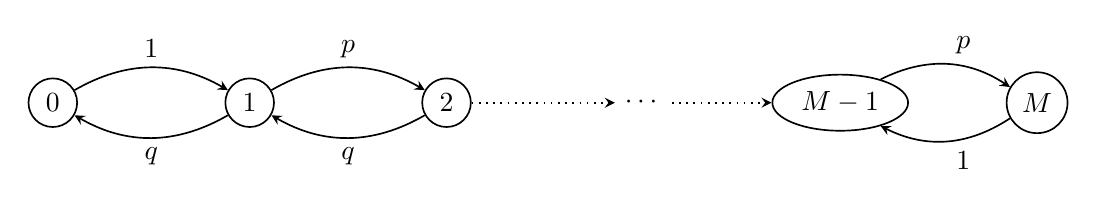
\begin{tikzpicture}[->, >=stealth, auto, semithick, node distance=2.5cm]
                \tikzstyle{every state}=[fill=white,draw=black,thick,text=black,scale=1]
                \node[circle, draw]    (A)                     {$0$};
                \node[circle, draw]    (B)[right of=A]   {$1$};
                \node[circle, draw]    (C)[right of=B]   {$2$};
                \node    (D)[right of=C]   {$\cdots$};
                \node[ellipse, draw]    (E)[right of=D]   {$M-1$};
                \node[circle, draw]    (F)[right of=E]   {$M$};

                \path
                (A) edge[bend left]  node{$1$}         (B)
                (B) edge[bend left]  node{$q$}         (A)
                (B) edge[bend left]  node{$p$}         (C)
                (C) edge[bend left]  node{$q$}         (B)
                (E) edge[bend left]  node{$p$}         (F)
                (F) edge[bend left]  node{$1$}         (E)
                (C) edge[dotted]     node{}            (D)
                (D) edge[dotted]     node{}            (E);
            \end{tikzpicture}
        \end{solution}
    \end{parts}

    \question{\textbf{11.37}}

    Consider a Markov chain with state space and the following transition
    probabilities:

    \(P_{jj + 1} = a_j\) and \(p_{j1} = 1 - a_j\) where \(0 < a_j < 1\)
    \begin{parts}
        \part Sketch the state transition diagram.
        \begin{solution}

            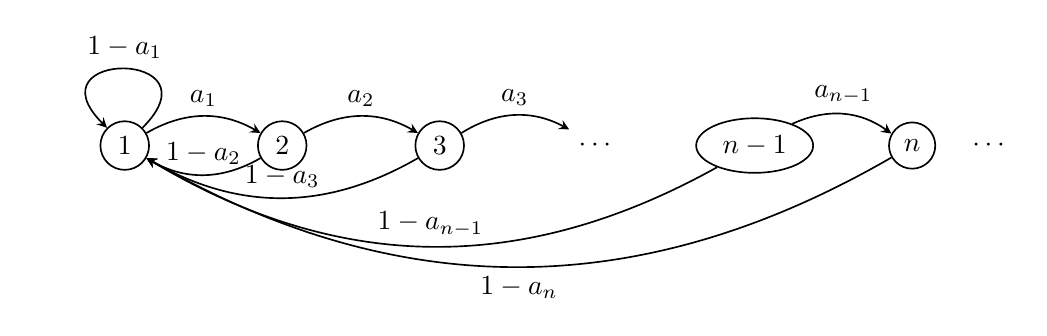
\begin{tikzpicture}[->, >=stealth, auto, semithick, node distance=2cm]
                \tikzstyle{every state}=[fill=white, draw=black, thick, text=black, scale=1]

                % Define the states
                \node[circle, draw] (1) {$1$};
                \node[circle, draw] (2) [right of=1] {$2$};
                \node[circle, draw] (3) [right of=2] {$3$};
                \node        (dots) [right of=3] {$\cdots$};
                \node[ellipse, draw] (n-1) [right of=dots] {$n-1$};
                \node[circle, draw] (n) [right of=n-1] {$n$};
                \node (dots2) [right of=n, node distance=1cm] {$\cdots$};

                % Connect the states with arrows
                \draw (1) to[bend left] node[midway, above] {$a_1$} (2);
                \draw (2) to[bend left] node[midway, above] {$a_2$} (3);
                \draw (3) to[bend left] node[midway, above] {$a_3$} (dots);
                % \draw (dots) to[bend left] node[midway, above] {$a_{n-1}$} (n-1);
                \draw (n-1) to[bend left] node[midway, above] {$a_{n - 1}$} (n);

                \draw (2) to[bend left] node[above] {$1-a_2$} (1);
                \draw (3) to[bend left] node[midway, above] {$1-a_3$} (1);
                \draw (n-1) to[bend left] node[midway, above] {$1-a_{n-1}$} (1);
                \draw (n) to[bend left] node[midway, below] {$1-a_{n}$} (1);

                \draw (1) to[loop] node[midway, above] {$1-a_1$} (1);

            \end{tikzpicture}
        \end{solution}

        \part Determine whether the Markov chain is irreducible.
        \begin{solution}
            The Markov chain is irreducible if there is a path from every state to every other state. In this case, there is a path from every state to every other state, so the Markov chain is irreducible.
        \end{solution}
    \end{parts}
\end{questions}

\end{document}
